%!TEX program = xelatex
\documentclass[dvipsnames, svgnames,a4paper,11pt]{article}
\usepackage{tikz}
\usetikzlibrary{calc}
\usepackage{eso-pic}
\AddToShipoutPictureBG{%
\begin{tikzpicture}[overlay,remember picture]
\draw[line width=0.6pt] % 边框粗细
    ($ (current page.north west) + (0.6cm,-0.6cm) $)
    rectangle
    ($ (current page.south east) + (-0.6cm,0.6cm) $); % 边框位置
\end{tikzpicture}}


\usepackage{xcolor}
\definecolor{c1}{HTML}{086173} % 目录颜色 原版为2752C9 紫灰色535AAA 蓝紫色0B0DB7 深蓝色070F94 湖绿色219394 松石灰绿086173
\definecolor{c2}{HTML}{E20129} % 引用颜色 原版\definecolor{c2}{RGB}{190,20,83} 橙色F24729

\usepackage{ctex}
\usepackage[top=28mm,bottom=28mm,left=15mm,right=15mm]{geometry}
\usepackage{hyperref} 
\hypersetup{
	colorlinks,
	linktoc = section, % 超链接位置,选项有section, page, all
	linkcolor = c1, % linkcolor 目录颜色
	citecolor = c1  % citecolor 引用颜色
}
\usepackage{amsmath,enumerate,multirow,float}
\usepackage{tabularx}
\usepackage{tabu}
\usepackage{subfig}
\usepackage{fancyhdr}
\usepackage{graphicx}
\usepackage{wrapfig}  
\usepackage{physics}
\usepackage{appendix}
\usepackage{amsfonts}

%
\usepackage{tcolorbox}
\tcbuselibrary{skins,breakable}
\newtcolorbox{tbox}[2][]{
    colframe=black!70!,
    breakable,
    enhanced,
	boxrule =0.5pt,
    title = {#2},
    fonttitle = \large\kaishu\bfseries,
	drop fuzzy shadow,
    #1
}
\newtcolorbox[auto counter,number within=section]{question}[1][]{
  top=2pt,bottom=2pt,arc=1mm,
  boxrule=0.5pt,
%   frame hidden,
  breakable,
  enhanced, %跨页后不会显示下边框
  coltitle=c1!80!gray,
  colframe=c1,
  colback=c1!3!white,
  drop fuzzy shadow,
  title={思考题~\thetcbcounter:\quad},
  fonttitle=\bfseries,
  attach title to upper,
  #1
}

% ---------------------------------------------------------------------
%	利用cleveref改变引用格式,\cref是引用命令
\usepackage{cleveref}
\crefformat{figure}{#2{\textcolor{c2}{Figure #1}}#3} % 图片的引用格式
\crefformat{equation}{#2{(\textcolor{c2}{#1})}#3} % 公式的引用格式
\crefformat{table}{#2{\textcolor{c2}{Table #1}}#3} % 表格的引用格式


% ---------------------------------------------------------------------
%	页眉页脚设置
\fancypagestyle{plain}{\pagestyle{fancy}}
\pagestyle{fancy}
\lhead{\kaishu 中山大学物理与天文学院近代物理实验\uppercase\expandafter{\romannumeral1}} % 左边页眉,学院 + 课程
\rhead{\kaishu 实验报告By黄罗琳} % 右边页眉,实验报告标题
\cfoot{\thepage} % 页脚,中间添加页码


% ---------------------------------------------------------------------
%	对目录、章节标题的设置
\renewcommand{\contentsname}{\centerline{\huge 目录}}
\usepackage{titlesec}
\usepackage{titletoc}
% \titleformat{章节}[形状]{格式}{标题序号}{序号与标题间距}{标题前命令}[标题后命令]
\titleformat{\section}{\centering\LARGE\songti}{}{1em}{}

% ---------------------------------------------------------------------
%   listing代码环境设置
\usepackage{listings}
\lstloadlanguages{python}
\lstdefinestyle{pythonstyle}{
backgroundcolor=\color{gray!5},
language=python,
frameround=tftt,
frame=shadowbox, 
keepspaces=true,
breaklines,
columns=spaceflexible,                   
basicstyle=\ttfamily\small, % 基本文本设置,字体为teletype,大小为scriptsize
keywordstyle=[1]\color{c1}\bfseries, 
keywordstyle=[2]\color{Red!70!black},   
stringstyle=\color{Purple},       
showstringspaces=false,
commentstyle=\ttfamily\scriptsize\color{green!40!black},%注释文本设置,字体为sf,大小为smaller
tabsize=2,
morekeywords={as},
morekeywords=[2]{np, plt, sp},
numbers=left, % 代码行数
numberstyle=\it\tiny\color{gray}, % 代码行数的数字字体设置
stepnumber=1,
rulesepcolor=\color{gray!30!white}
}




% ---------------------------------------------------------------------
%	其他设置
\def\degree{${}^{\circ}$} % 角度
\graphicspath{{./images/}} % 插入图片的相对路径
\allowdisplaybreaks[4]  %允许公式跨页 
\usepackage{lipsum}
\usepackage{adjustbox}
%\usepackage{mathrsfs} % 字体
%\captionsetup[figure]{name=Figure} % 图片形式
%\captionsetup[table]{name=Table} % 表格形式
\begin{document}
	
	% 实验报告封面	
	% 顶栏
	\begin{table}
		\renewcommand\arraystretch{1.7}
		\begin{tabularx}{\textwidth}{
				|X|X|X|X
				|X|X|X|X|}
			\hline
			\multicolumn{2}{|c|}{预习报告}&\multicolumn{2}{|c|}{实验记录}&\multicolumn{2}{|c|}{分析讨论}&\multicolumn{2}{|c|}{总成绩}\\
			\hline
			\LARGE25 & & \LARGE25 & & \LARGE30 & & \LARGE80 & \\
			\hline
		\end{tabularx}
	\end{table}
	% ---
	
	% 信息栏
	\begin{table}
		\renewcommand\arraystretch{1.7}
		\begin{tabularx}{\textwidth}{|X|X|X|X|}
			\hline
			年级、专业: & 2022级 物理学 &组号: & \\
			\hline
			姓名: & 黄罗琳、王显   & 学号: &  22344001、22344002 \\
			\hline
			实验时间: & 2024/9/20 & 教师签名: & \\
			\hline
		\end{tabularx}
	\end{table}
	% ---
	
	% 大标题
	\begin{center}
		\LARGE D1 \quad 锁相放大器与弱信号测量
	\end{center}
	% ---
	
	% 注意事项
	
	% 基本
	\textbf{【实验报告注意事项】}
	
		\begin{enumerate}
			\item 预习报告:课前认真研读实验讲义,弄清实验原理;实验所需的仪器设备、用具及其使用、完成课前预习思考题;了解实验需要测量的物理量,并根据要求提前准备实验记录表格。
			\item 实验记录:认真、客观记录实验条件、实验过程中的现象以及数据。实验记录请用珠笔或者钢笔书写并签名(\textcolor{red}{\textbf{用铅笔记录的被认为无效}})。\textcolor{red}{\textbf{保持原始记录,包括写错删除部分,如因误记需要修改记录,必须按规范修改。}}(不得输入电脑打印,但可扫描手记后打印扫描件);离开前请实验教师检查记录并签名。
			\item 数据处理及分析讨论:处理实验原始数据(学习仪器使用类型的实验除外),对数据的可靠性和合理性进行分析;按规范呈现数据和结果(图、表),包括数据、图表按顺序编号及其引用;分析物理现象(含回答实验思考题,写出问题思考过程,必要时按规范引用数据);最后得出结论。
		\end{enumerate}
		
		
	
		
	

	
	% 安全
		
	 \textbf{本实验报告阅读说明}:
		\begin{enumerate}
			\item 本实验报告基于基本实验原理,尽可能符合逻辑,并且保证实验所有要求的内容均有结果或解释,如果出现超出能力范围,会进行理论建模进行相关说明。
			\item 本实验报告由组内人员共同完成,所有分工合作均保证工作量尽可能平均,如有特殊情况会在结语处进行说明。
			\item 本实验报告会于实验课程结束后上传至GitHub开源,相关仓库包括基础物理实验、电子技术实验,可供查阅。
		\end{enumerate}
	% 目录
	\clearpage
	\tableofcontents
	\clearpage
	% ---
	
	
	
	% 预习报告	
	
	% 小标题
	\setcounter{section}{0}
	\section{D1 锁相放大器与弱信号测量 \quad\heiti 原理背景}
	% ---
	
	% 实验目的
	\subsection{实验原理基础}
	\subsubsection{实验问题背景}
	现代信号测量中,面对微弱信号(如毫伏级)的情况下,传统示波器常难以区分信号与噪声。此时,锁相放大器(Lock-in Amplifier)通过提取特定频率成分,显著提高了弱信号测量的精度,尤其适用于噪声淹没信号的实验。

锁相放大器的高效使用要求理解其工作原理,包括相干检测、参考信号、混频及低通滤波等技术,并正确设置增益、时间常数和参考频率等参数。一般测量关注信号而忽视噪声,但在精密测量领域,噪声本身亦可成为研究对象。锁相放大器不仅能放大信号,还可用于噪声分析,如频谱分布及信噪比(SNR)测量。

\subsubsection{信噪比与信噪改善比}

信噪比(Signal-to-Noise Ratio, SNR)

信噪比是表示信号强度与噪声强度之间关系的一个度量,它用来衡量有用信号相对于背景噪声的强弱程度。信噪比越高,表示信号相对于噪声越强,信号质量也越好。信噪比通常以分贝(dB)为单位,公式如下:

\[
SNR = 10 \cdot \log_{10} \left( \frac{P_{signal}}{P_{noise}} \right)
\]

其中,\(P_{signal}\) 是信号的功率,\(P_{noise}\) 是噪声的功率。

在许多应用中,如通信系统、音频处理和图像处理,信噪比是评估系统性能的重要指标。

信噪改善比(Signal-to-Noise Improvement Ratio, SNIR)

信噪改善比: 是对信噪比的改善程度的度量。它用来表示通过某种方法(例如滤波、降噪算法等)对信噪比的提升效果。信噪改善比越大,意味着该方法有效地增强了信号质量或减少了噪声。

信噪改善比可以通过对比处理前后的信噪比来计算:

\[
SNIR = SNR_{\text{after}} - SNR_{\text{before}}
\]

其中,\(SNR_{\text{before}}\) 是处理前的信噪比,\(SNR_{\text{after}}\) 是处理后的信噪比。该值通常以分贝(dB)为单位。


\subsubsection{滤波法提升信噪比}

RC低通滤波器是一种简单而有效的方法,通过降低高频噪声成分来改善信噪比(SNR)。它广泛应用于信号处理和电子电路中。


一阶RC低通滤波器的传递函数为:

\begin{equation}
H(\omega) = \frac{1}{1 + j\omega RC}
\end{equation}

其中:
\begin{itemize}
    \item \( \omega \) 是信号的角频率,
    \item \( R \) 是电阻,
    \item \( C \) 是电容。
\end{itemize}

传递函数的幅度,即增益为:

\begin{equation}
|H(\omega)| = \frac{1}{\sqrt{1 + (\omega RC)^2}}
\end{equation}

在低频时(\( \omega \rightarrow 0 \)),增益接近1,意味着信号以最小的衰减通过。在高频时(\( \omega \rightarrow \infty \)),增益接近0,表示高频成分被严重衰减。

截止频率 \( \omega_0 \) 是输出信号幅度减少3 dB(约70.7\%的输入信号)时的频率。其定义为:

\begin{equation}
\omega_0 = \frac{1}{RC}
\end{equation}

通过选择适当的 \( R \) 和 \( C \) 值,可以控制滤波器的频率响应。


为了获得更陡的频率响应,可以将多个RC低通滤波器级联。 \( n \) 级RC低通滤波器的总传递函数为:

\begin{equation}
H(\omega)^n = \left( \frac{1}{1 + j\omega RC} \right)^n
\end{equation}

每个级提供额外的高频成分衰减,进一步通过滤除更多噪声来改善信噪比。
\begin{figure}[{H}]
	\centering
	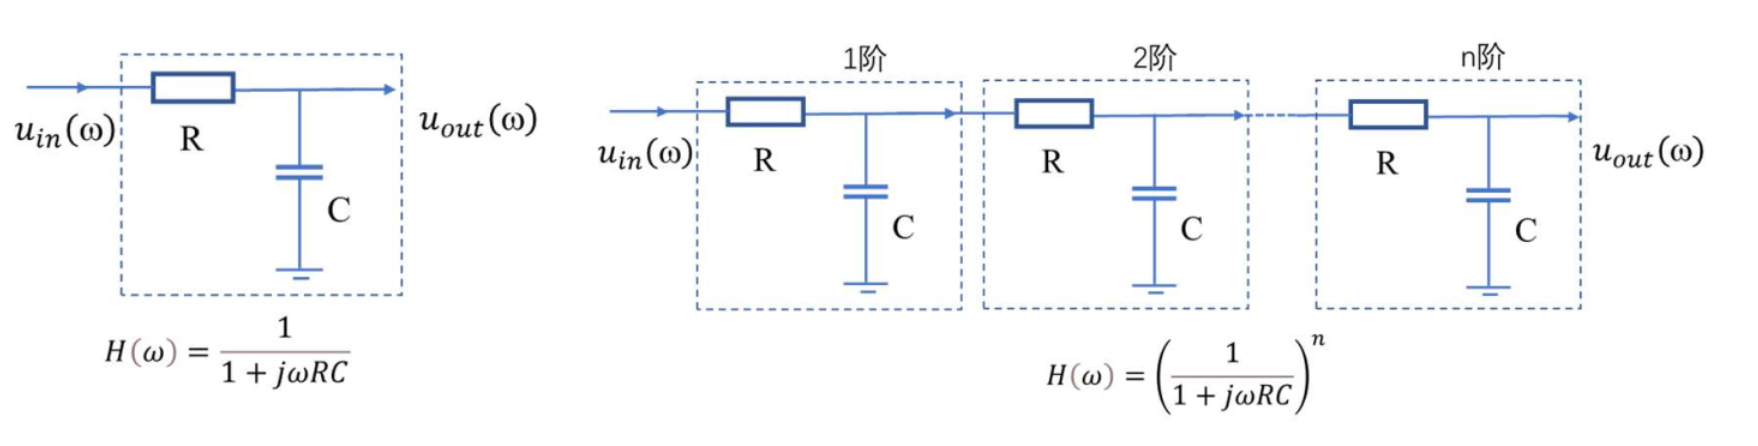
\includegraphics[width=1\linewidth]{原理1.png}
	\caption{多个RC低通滤波器级联}
	\label{}
\end{figure}
\subsubsection{锁相放大法提升信噪比}
锁相放大法(Lock-in Amplification)是一种高灵敏度信号检测技术,广泛应用于物理、电子工程和其他科学领域,尤其在测量微弱信号时表现突出。其基本原理和工作步骤如下:

锁相放大法通过调制和解调的方式,将待测信号从噪声中提取出来。其核心在于使用相敏检测技术,这使得该方法能够有效地隔离信号与噪声。

工作步骤
\begin{enumerate}
	\item 信号调制:将待测的微弱信号 \( s(t) \) 与一个高频正弦载波 \( \cos(𝜔ₘ t) \) 相乘。这一过程将信号频谱迁移至调制频率 \( 𝜔ₘ \) 附近。这种频谱迁移有助于避免低频噪声(如1/f噪声)的干扰。
	\item 相敏检波:使用相敏检波器(PSD)对调制后的信号进行解调。PSD能够通过参考信号(与调制信号同频且相位相同)提取目标信号。由于噪声的相位通常不同于信号,因此噪声的影响被显著降低。
	\item 低通滤波:将解调后的信号通过一个窄带低通滤波器(LPF),进一步去除高频噪声和不必要的频率成分。低通滤波器的带宽设计得非常窄,使得只有调制频率附近的信号能通过,从而提高信噪比。
\end{enumerate}
\subsection{锁相放大器工作原理}
锁相放大器的基本结构如图 2(b) 和 (c) 所示的虚线框内, 其中信号通道、参考通道为锁相放大器的输入通道,相敏检测器(PSD)和低通滤波器(LPF)等。

\begin{figure}[{H}]
	\centering
	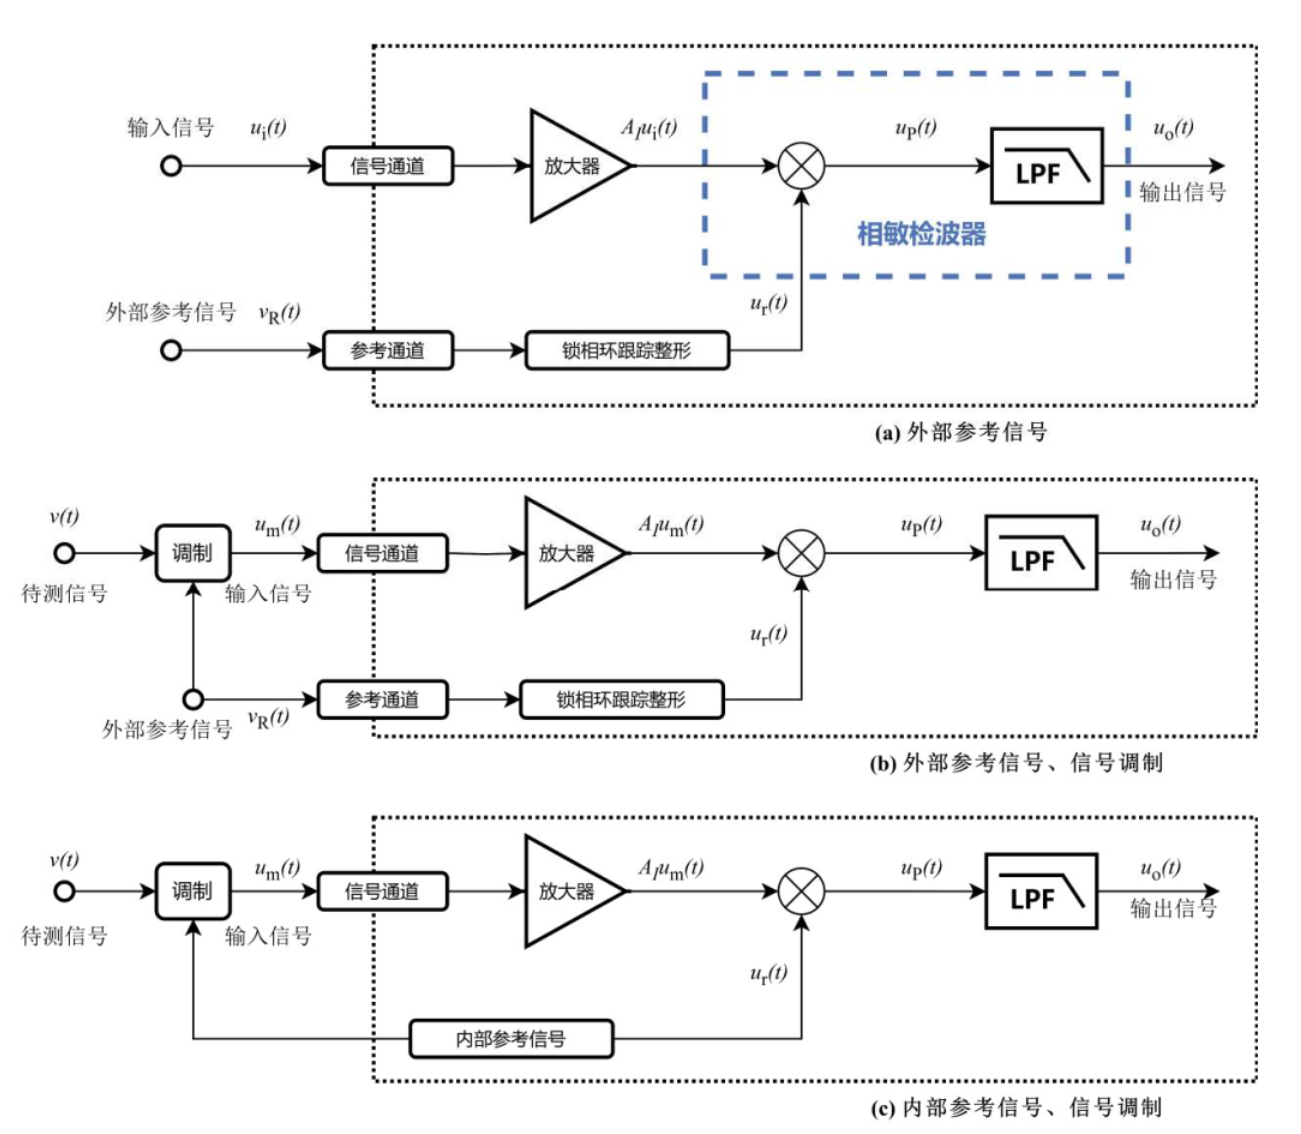
\includegraphics[width=0.8\linewidth]{原理2.png}
	\caption{锁相放大器的工作原理}
	\label{}
\end{figure}


对于三角函数信号 \(u_i(t) = u_0 \sin (\omega_s t + \phi)\),可直接从信号通道输入(虚线框内的)锁相放大器,此时待测信号即为锁相放大器的输入信号。对于非三角函数信号或慢变信号(如直流信号),它在输入锁相放大器前,需要被与参考信号频率相同的正弦信号所调制。原则上,参考信号既可以是外部输入信号 \(v_R(t)\) 经整定后得到的正弦信号,也可以是锁相放大器内部自带参考信号源提供的正弦信号。实际操作上,因外部输入的参考信号不可避免地受到干扰和变形,要求锁相环对外部信号有很强的整定能力。为改善信号处理效果,现在的锁相放大器内部都有自带的参考信号,且使用内部参考信号的效果优于外部参考信号。

三角函数信号可视为被调制的直流信号。一般情况下,下面以非三角函数信号为待测信号,使用数学方式阐述锁相放大器的工作原理。对于噪声,它可以叠加在调制前的信号中,也可以叠加在调制后的信号中;锁相放大器信号输入端不能区分这两种情况,因此,下面推导中只考虑后者,即输入信号为三角函数,输入噪声为 \(n(t)\)。

调制前信号包含待测信号和噪声,有:
\begin{equation}
    v(t) = s(t) + n(t)
\end{equation}

经 \(\sin (\omega_m t + \theta)\) 信号调制后:
\begin{equation}
    u_m(t) = x(t) \sin (\omega_m t + \theta) = s(t) \sin (\omega_m t + \theta) + n(t)
\end{equation}
其中, \(n(t) = v_N(t) \sin (\omega_m t + \theta)\)。

\begin{enumerate}
    \item 输入:式(8)给出了锁相放大器的输入信号 \(u_{\text{in}}(t)\)。
    \item 放大:输入信号仍然很弱,在经前置放大器后被放大 \(A_I\) 倍:
    \begin{equation}
        u_a(t) = A_I s(t) \sin (\omega_m t + \theta) + A_I n(t)
    \end{equation}
    此时,信号与噪声都被同时放大了。
    \item 解调:锁相放大器采用参考信号 \(u_r(t) = \sin (\omega_r t)\) 解调:
    \begin{equation}
        u_{px}(t) = u_r(t) u_s(t) = A_I [s(t) \sin (\omega_m t + \theta) \sin (\omega_r t) + n(t) \sin (\omega_r t)]
    \end{equation}
    \[
        = A_I \left\{s(2t) \left[\cos ((\omega_m - \omega_r) t + \theta) - \cos ((\omega_m + \omega_r) t + \theta)\right] + n(t) \sin (\omega_r t)\right\}
    \]

    对于调制信号是通过某种物理机制由参考信号触发或用参考信号本身情况,参考信号与调制信号频率相同 (\(\omega_m = \omega_r\)),相位差 \(\theta\) 确定;并经过理想的低通滤波器滤去高频分量,则滤波器输出信号为:
    \begin{equation}
        u_{ox}(t) = A_I \left[\frac{1}{2} s(t) \cos \theta + n_x(t)\right]
    \end{equation}
    式中,\(n_x(t)\) 为未被滤去的、与参考频率相同的“同频噪声”,一般情况下其幅值远小于信号,即对高信噪比情况:
    \begin{equation}
        u_{ox}(t) = s_{ox}(t) = \frac{1}{2} A_I s(t) \cos \theta
    \end{equation}
    锁相放大器输出信号 \(s(t)\) 有效值:
    \begin{equation}
        X = \frac{\sqrt{2} u_{ox}(t)}{A_I} = R \cos \theta
    \end{equation}

    为了获得完整的输入信号,需采用另一路频率相同、且与参考信号相位相差 \(\pi/2\) 的信号 \(u_{r1}(t) = \cos (\omega_r t)\) 作为解调信号, 则通过相敏检测后此路信号与另一路信号也相差 \(\pi/2\):
    \begin{equation}
        s_{py}(t) = \frac{1}{2} A_I s(t) \left[\sin ((\omega_m - \omega_r) t + \theta) + \sin ((\omega_m + \omega_r) t + \theta)\right]
    \end{equation}
    \begin{equation}
        s_{oy}(t) = \frac{1}{2} A_I s(t) \sin \theta
    \end{equation}
    \[
        Y = \frac{\sqrt{2} u_{oy}(t)}{A_I} = R \sin \theta
    \]
    \begin{equation}
        R = \sqrt{X^2 + Y^2}
    \end{equation}
    定义锁相放大器输入信号相对于解调信号(图 3 的参考信号)的相位差:
    \begin{equation}
        \theta = \tan^{-1} \frac{u_{oy}(t)}{u_{ox}(t)}
    \end{equation}
    这种可同时测量完整输入信号信息的锁相放大器称双相锁相放大器。
\begin{figure}[{H}]
	\centering
	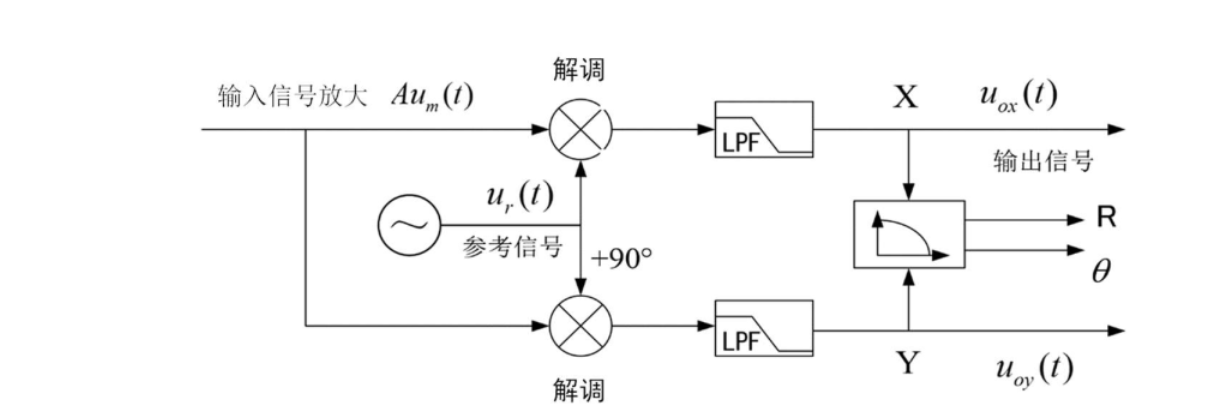
\includegraphics[width=0.8\linewidth]{原理3.png}
	\caption{双锁相放大器}
	\label{}
\end{figure}
    \item 然而,实际滤波器并不理想,且滤波器的性能与锁相放大器参数设置(选择)有关。要用好锁相放大器,就需要对滤波器的工作原理有更深入的了解。先讨论未被滤波(时间常数很小)时,从式(10)和式(14):
    \begin{equation}
        R(t) = s(t) |\sin (\omega_m t + \theta)|
    \end{equation}
    即信号项被 \(|\sin (\omega_m t + \theta)|\) 所调制,其频率是被调制信号频率 \(\omega_m\) 的 2 倍。对 \(|\sin (\omega_m t + \theta)|\) 做傅里叶变换,可得到该频谱,即 2\(\omega_m\) 频率下的幅值和直流分量(平均值)。在信噪比较高时,此式容易被观察到。
\end{enumerate}
\subsection{名称由来}

在许多应用场合中,锁相放大器的参考信号是由外部设备提供的,例如光学斩波器或信号发生器。这种工作模式称为“外部参考模式”(external reference mode)。在这种模式下,锁相放大器的参考通道会接收外部输入的参考信号,并对其进行放大和整形。参考信号通常是正弦波或近似正弦波的周期信号,可能由于噪声或失真而有所变形。为确保后续信号处理的准确性,锁相放大器首先会通过放大器和整形电路将该外部信号处理为一个更为标准、纯净的信号,去除掉噪声和畸变的影响。

在信号整形之后,锁相放大器会使用锁相环(Phase-Locked Loop,简称PLL)技术对外部输入的参考信号进行频率和相位的跟踪。这意味着锁相环会根据输入参考信号产生一个与其频率相同、且相位差锁定的正弦信号。这个锁相环生成的信号即是图 D1-7(b) 所示的 \( u_r(t) \)。这个新生成的参考信号相当于一个理想的版本,保留了外部参考信号的主要特性(如频率),但消除了由于干扰或噪声引起的畸变。这样,锁相放大器可以在保持参考信号准确性的同时,进行高精度的信号检测和分析。

“锁相”的概念在这里指的是:通过锁相环(PLL),锁定外部参考信号与内部生成的参考信号之间的相位关系,确保两者具有相同的频率和确定的相位差。相位差的锁定是锁相放大器实现相敏检测(phase-sensitive detection,PSD)的基础。相敏检测是锁相放大器的核心功能,它允许设备通过与参考信号进行比较,检测到与输入信号同步的部分,滤除掉不相关的噪声和干扰成分,从而提高信号测量的精度。

使用外部参考信号时,锁相放大器能够灵活地处理各种不同来源的周期性信号。这在实际应用中非常有用,尤其是当测量系统中使用的信号源(如光学斩波器或信号发生器)已经包含了周期性参考信号时。通过外部参考模式,锁相放大器能够自动与这些外部参考信号同步,不仅保持了与外部设备的协调性,还避免了因噪声或相位漂移导致的测量误差。

总体而言,锁相放大器的外部参考模式使得其在多种复杂环境下的应用成为可能。无论是光学实验、无线电频率测量,还是其他需要高灵敏度信号检测的领域,锁相放大器都可以通过精确锁定外部参考信号,实现高效的信号提取和测量。这也是锁相放大器在科研和工业测试中的广泛应用的关键所在。

	\subsection{原理部分思考题}
	
	% 思考题1
	\begin{question}
		市频 50Hz 干扰通常通过电源耦合,影响仪器的测量结果;对于 997Hz 的待测信号,
50Hz 干扰是噪声吗?对锁相放大器的测量会有影响吗?
	\end{question}
	50Hz 的市频干扰对于 997Hz 的待测信号确实是噪声,但为避开市电 50Hz 及其整数倍频率外部干扰,
待测信号选择了 997Hz,因此对于锁相放大器而言测量几乎不存在影响。
	% 思考题2
	\begin{question}
		如何用锁相放大器检测到待测的直流信号或慢变信号?
	\end{question}
	在锁相放大器的使用中,首先需要对待测信号 \(x(t)\) 的频谱进行迁移,即进行调制。其调制过程是将待测信号 \(x(t)\) 乘以频率为 \(\omega_0\) 的正弦载波。例如,待测信号可以表示为:
\[
x(t) = s(t) + n(t)
\]
经过信号 \(\sin(\omega_0 t + \theta)\) 调制后,变为:
\[
u(t) = x(t) \sin(\omega_0 t + \theta) = s(t) \sin(\omega_0 t + \theta) + n(t) \sin(\omega_0 t + \theta)
\]
从而将其频谱迁移到调制频率 \(\omega_0\) 附近。

接下来,对信号进行选频放大处理,并使用相敏检测器对信号进行解调,将其频移到直流的两侧。之后,通过窄带低通滤波器滤除噪声,得到高信噪比的放大信号。这样,锁相放大器就能够检测到待测直流信号或慢变信号。

	% 思考题3
	\begin{question}
		如用斩波器调制直流信号(如光强),被斩制后的信号仍
然包含有直流分量(即平均值不为零),但该直流分量随交流信号输入锁相放大器后
不会被锁相放大器检测,请从数学推导上说明。
	\end{question}
	被斩波器调制后的信号为:
\[
A(t) = u_m(t) + a = [s(t) + n(t)] \sin(\omega_0 t + \theta) + a
\]
其中 \(a\) 为直流分量。经过锁相放大器后得到:
\[
B(t) = A_l [s(t) + n(t)] \sin(\omega_0 t + \theta) + A_l a
\]
此处 \(A_l\) 为锁相放大器的放大倍数,之后再经过参考信号 \(u_r(t) = \sin(\omega_0 t)\) 解调得到信号:
\[
B(t) = \frac{A_l}{2} [s(t) + n(t)] (\cos \theta - \cos(2 \omega_0 t + \theta)) + A_l a \sin(\omega_0 t)
\]
这里 \(\omega_0\) 为高频频率,因此经过低通滤波后,低频分量 \(\frac{A_l}{2} [s(t) + n(t)] \cos \theta\) 得到保留,而高频分量 \(\frac{A_l}{2} [s(t) + n(t)] \cos(2 \omega_0 t + \theta)\) 以及 \(A_l a \sin(\omega_0 t)\) 将被滤过。由此可见,直流分量会被过滤而不会被放大。

此外,若 \(a\) 为慢变信号,不妨设 \(a = \sin(\omega_1 t)\),则其经过解调后变为:
\[
A_l \sin(\omega_1 t) \sin(\omega_0 t) = \frac{A_l}{2} [\cos(\omega_1 t - \omega_0 t) - \cos(\omega_1 t + \omega_0 t)]
\]
此时两个信号也都是高频信号(\(\omega_1\) 的值非常小),经过低通滤波器后均会被滤去,因此直流分量随交流信号输入锁相放大器后不会被锁相放大器检测到。


	\begin{question}
		相位以及相位差的含义是什么?锁相放大器输出的是待测信号的相位还是待测信号
与参考信号之间的相位差?
	\end{question}
	相位是交流信号中的相角,例如信号 \(x(t) = A e^{i(\omega t + \phi)}\) 的相位为 \(\phi\)。相位差是指两个交流信号的相位之差。设两个交流信号分别为:
	\[
	x_1(t) = A e^{i(\omega t + \phi_1)}, \quad x_2(t) = A e^{i(\omega t + \phi_2)}
	\]
	则两个交流信号的相位差为:
	\[
	\phi_1 - \phi_2
	\]
	锁相放大器输出的 \(\theta\) 是待测信号与参考信号之间的相位差。

	\begin{question}
		(选)以上仅讨论了滤波器的幅频特性,那么其相频特性又会是怎样呢?在时域的时
间响应特性又是怎样呢?感兴趣的同学可以自己推导。进一步,该相频特性会影响到
相位角$\theta$的测量吗?
	\end{question}
	锁相放大器的相频特性为:
	\[
	\Delta \theta = \frac{L}{v} \times 2\pi f
	\]

	该特性会影响相位角 \(\theta\) 的测量。

	% ---
	
	
	
	% 实验记录	
	\clearpage
	\section{D1 锁相放大器与弱信号测量(1) \quad\heiti 预习报告}
	% ---
	
	% 实验目的
	\subsection{实验目的}
	\begin{enumerate}
		\item 了解锁相放大器工作原理和特点,理解信号、噪声、信噪比等概念。
		\item 掌握锁相放大器基本参数含义及锁相放大器的基本操作,学会合理选择或调节参数(频
		率、相位、灵敏度、时间常数、陡降);复习示波器的使用;
		\item 掌握用锁相放大器检测弱信号方法,通过与示波器比较其检测能力了解其技术优势。
	\end{enumerate}
	% ---
	\subsection{实验要求}
	\begin{enumerate}
		\item 把锁相放大器作为测量工具,理解其工作原理:
		\begin{enumerate}
			\item 基本概念:信号、噪声、信噪比;时域谱、频域谱;
			\item 锁相放大器工作原理:信号的调制、解调(相敏检波)、滤波的数学表述;
		\end{enumerate}
		
		\item 学习合理地设置锁相放大器参数,为后面实验应用锁相放大器及时、准确、精密地
		获得待测微弱信号的之间获得合理的平衡。锁相放大器参数(频率、相位、灵敏
		度、时间常数、陡降)及其对锁相放大器测量的影响;
	
		\item 锁相放大器操作:参数设置,用示波器观察锁相放大器通道输出结果,或用
		DISPLAY 显示输出结果;
		
		\item 在实验报告中用实验结果回答问题。
		
		\item (选)参数设置和操作:浮地,差分(A-B)输入,外部输入参考信号(TTL 参考
		信号),扫频。
		
	\end{enumerate}
	% 仪器用具
	\subsection{仪器用具}
	\begin{tabular}{|c|m{4cm}|c|m{6cm}|c|}
		\hline
		编号 & 仪器用具名称 & 数量 & 主要参数(型号,规格等) & 备注 \\
		\hline
		1 & 锁相放大器 & 1 & OE1022(系列) &  \\
		\hline
		2 & 配套教学实验箱 & 1 &  &  \\
		\hline
		3 & 示波器 & 1 & RIGOL DS2202A &  \\
		\hline
		4 & 信号发生器 & 1 & RIGOL DG4162 &  \\
		\hline
		5 & BNC-BNC 信号线 & 若干 &  &  \\
		\hline
		\end{tabular}
	

	
	
	
	% 实验前思考题
	\subsection{预习思考题题}
	
	% 思考题1
	\begin{question}
		噪声有哪些类型?一般测量对象本身的噪声是哪来的?它有什么特征?
	\end{question}
	噪声可分为来自外界的环境的有规律的声源(如市电噪声)以及来自被测量对象本身的噪声(如无规
的热噪声)。
对于一项实验,一般测量对象本身的噪声,最典型的比如无规的热噪声,既可来自于实验对象本身,也
可来自于测量系统,包括传感器和测量仪器。
	% 思考题2
	\begin{question}
		是否可以用 RIGOL DG4162 信号发生器产生白噪声取代教学实验箱产生的白噪声?如
何将它与信号混合?
	\end{question}
	可以用 RIGOL DG4162 信号发生器产生白噪声取代教学实验箱产生的白噪声。
按 Utility -> CH1 设置 -> 噪声叠加,用户可以打开或关闭噪声叠加功能。默认为“关闭”。选择“打
开”时,可以使用数字键盘或方向键和旋钮设置噪声比例。可设置范围为 0\% 至 50\%,默认值为 10.0\%。
当 Mod、 Sweep 或 Burst 开启时,噪声叠加菜单置灰禁用。
本实验中并未进行此操作,只是通过查阅 RIGOL DG4162 用户手册得知上述操作步骤。

	
	
	
	% 实验记录	
	\clearpage
	% 顶栏
	\begin{table}
		\renewcommand\arraystretch{1.7}
		\centering
		\begin{tabularx}{\textwidth}{|X|X|X|X|}
			\hline
			专业: & 物理学 & 年级: & 2022级 \\
			\hline
			姓名: &  & 学号: & \\
			\hline
			室温: &  & 实验地点: & A522 \\
			\hline
			学生签名:& 见\textbf{附件}部分 & 评分: &\\
			\hline
			实验时间:& 2024// & 教师签名:&\\
			\hline
		\end{tabularx}
	\end{table}
	% ---
	
	% 小标题
	\section{ D1 锁相放大器与弱信号测量(1)\quad\heiti 实验记录}
	% ---
	
	% 实验过程记录
	\subsection{实验内容、步骤与结果}
	
	%
	\subsubsection{操作步骤记录}
	\begin{enumerate}
		\item 开始实验前,激光器要预热大约一个小时,以免发生波长振动。
		\item 搭建光路,如示意图所示,相关距离参数见手绘图。
		\item 确认光路中物光和参考光的光程差大致相等;物光和参考光夹角(30-50° );物光和参考
		光光强比 3:1-5:1。
		\item 设定曝光时间进行曝光(注意在整个曝光时间内尽量避免走动及大声说话)。
		\item 拍摄完毕以后,全息片要经过显影、停影、定影、水漂及晾干等四个步骤以后才能观察
		再现,整个操作过程均应在暗绿灯下进行,但要认真保持清洁。
		\item 把制作好的全息片放回原来位置(乳胶面仍对
		着光),从底片后面观察再现的虚像。

	\end{enumerate}	
	
	%
	\subsubsection{}
	\begin{enumerate}
		\item \begin{table}[h]
			\centering
			\caption{表格示例}
			\label{tab:tab1}
			\begin{tabular}{|c|c|c|c|c|c|}
				\hline
				组1/序号i & 1 & 2 & 3 & 4 & 5 \\
				$v_{1i}(m/s)$ & 1.26 & 1.08 & 1.00 & 0.75 & 0.38 \\
				$f_{1i}(Hz)$ & 40073 & 40127 & 40105 & 40088 & 40066 \\
				\hline
				组2/序号i & 1 & 2 & 3 & 4 & 5 \\
				$v_{2i}(m/s)$ & 1.21 & 1.06 & 0.99 & 0.52 & 0.57 \\
				$f_{2i}(Hz)$ & 40143 & 40125 & 40084 & 40080 & 40067 \\
				\hline
				组3/序号i & 1 & 2 & 3 & 4 & 5 \\
				$v_{3i}(m/s)$ & 1.15 & 0.98 & 0.78 & 0.59 & 0.36 \\
				$f_{3i}(Hz)$ & 40135 & 40115 & 40092 & 40070 & 40044 \\
				\hline
			\end{tabular}
		\end{table}		
	\end{enumerate}
	
	% ---
	
	% 原始数据
	\clearpage
	\subsection{原始数据记录}
	实验记录本上的原始数据见%\cref{}(签字)。
	
	实验台桌面整理见%\textbf{附件}部分(\cref{})。
	
	其它原始数据见%\cref{}。
	% ---
	
	% 问题记录
	\subsection{实验过程遇到问题及解决办法}
	\begin{enumerate}
		\item 
	\end{enumerate}
	% ---
	
	
	
	% 分析与讨论	
	\clearpage
	
	% 顶栏
	\begin{table}
		\renewcommand\arraystretch{1.7}
		\begin{tabularx}{\textwidth}{|X|X|X|X|}
			\hline
			专业:& 物理学 &年级:& 2022级\\
			\hline
			姓名: &  & 学号:& \\
			\hline
			日期:&  & 评分: &\\
			\hline
		\end{tabularx}
	\end{table}
	% ---
	
	% 小标题
	\section{D1 锁相放大器与弱信号测量(1)\quad\heiti 分析与讨论}
	% ---
	
	% 数据处理
	\subsection{实验数据分析}
	
	%
	\subsubsection{}
	\begin{enumerate}
		\item 
	\end{enumerate}
	
	%
	\subsubsection{}
	\begin{enumerate}
		\item 
	\end{enumerate}
	
	%
	\subsubsection{}
	
	% ---
	
	% 实验后思考题
	\subsection{实验后思考题}
	
	%思考题1
	\begin{question}
		
	\end{question}
	
	% 思考题2
	\begin{question}
		
	\end{question}
	
	% 思考题3
	\begin{question}
		
	\end{question}
	
	% ---
	
	
	% 结语部分
	\clearpage
	
	% 小标题
	\section{ETX 实验名称××× \quad\heiti 结语}
	% ---
	
	% 总结、杂谈与致谢
	\subsection{实验心得和体会、意见建议等}
	\begin{enumerate}
		\item 
	\end{enumerate}
	% ---
	

	% 附件
	\subsection{附件及实验相关的软硬件资料等}
	试验台桌面整理如%\cref{}所示。
	
	实验报告个人签名如

	% ---
	
	
\end{document}